\section{Evaluation}
\label{sec:evaluation}

This chapter evaluates the first iteration of the aBridgeAI system across three dimensions: frontend user experience (Section~\ref{sec:eval_frontend}), backend performance under load (Section~\ref{sec:eval_backend}), and AI model comparison for quiz generation (Section~\ref{sec:eval_ai_model}).

% ===========================================================
\subsection{Frontend Evaluation}
\label{sec:eval_frontend}

Frontend quality is assessed using Google Lighthouse, an industry-standard automated auditing tool that evaluates web pages across four categories: Performance, Accessibility, Best Practices, and SEO. Each page is tested in mobile emulation mode (simulated throttling) to reflect real-world conditions.

Table~\ref{tab:lighthouse_results} presents the Lighthouse audit results for the primary user-facing pages of the aBridgeAI frontend.

\begin{table}[htbp]
\centering
\caption{Lighthouse Audit Results (Mobile, Simulated Throttling)}
\label{tab:lighthouse_results}
\renewcommand{\arraystretch}{1.3}
\begin{tabular}{|l|c|c|c|c|}
\hline
\textbf{Page} & \textbf{Performance} & \textbf{Accessibility} & \textbf{Best Practices} & \textbf{SEO} \\
\hline
Login                  & 98 & 95 & 100 & 100 \\
Student Dashboard      & 97 & 100 & 100  & 100  \\
\hline
\end{tabular}
\end{table}

\paragraph{Login Page}

Figure~\ref{fig:lighthouse_login} shows the Lighthouse report for the Login page.

\begin{figure}[H]
    \centering
    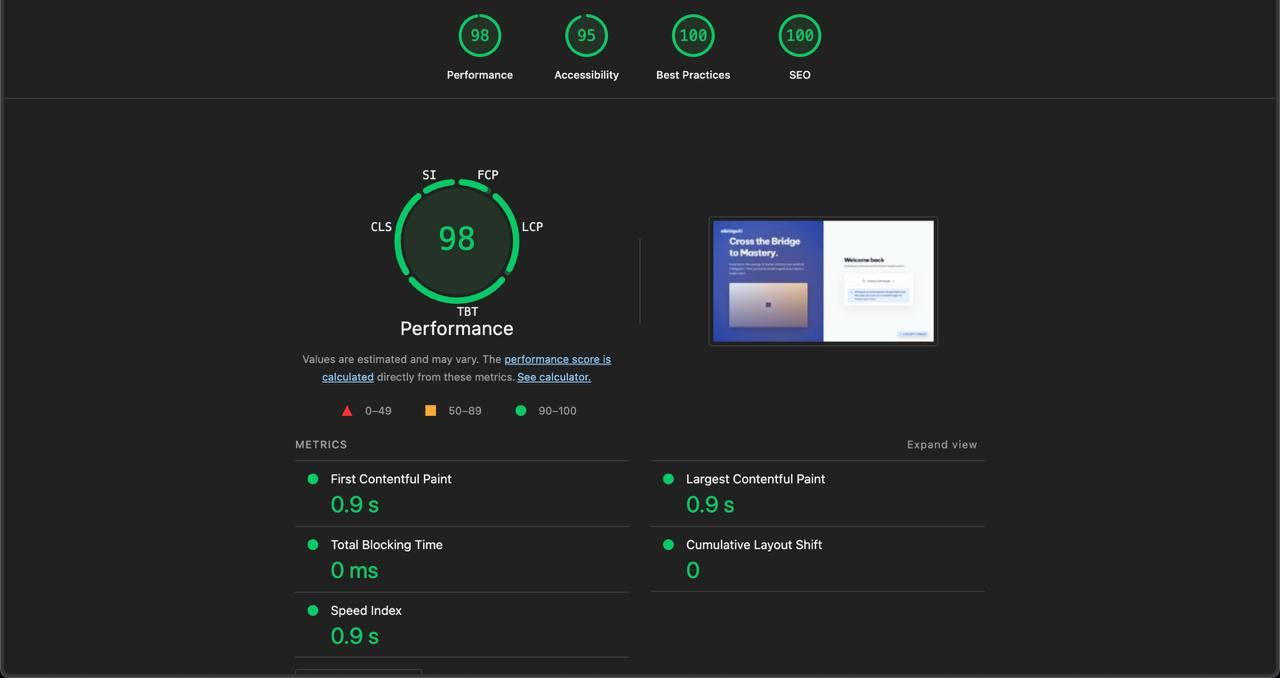
\includegraphics[width=0.85\textwidth]{graphics/lighthouse_login.jpg}
    \caption{Lighthouse audit results for the Login page.}
    \label{fig:lighthouse_login}
\end{figure}

Key performance metrics:
\begin{itemize}
    \item First Contentful Paint (FCP): 0.9\,s
    \item Largest Contentful Paint (LCP): 0.9\,s
    \item Total Blocking Time (TBT): 0\,ms
    \item Cumulative Layout Shift (CLS): 0
    \item Speed Index: 0.9\,s
\end{itemize}

\paragraph{Student Dashboard}

Figure~\ref{fig:lighthouse_dashboard} shows the Lighthouse report for the Student Dashboard page.

\begin{figure}[H]
    \centering
    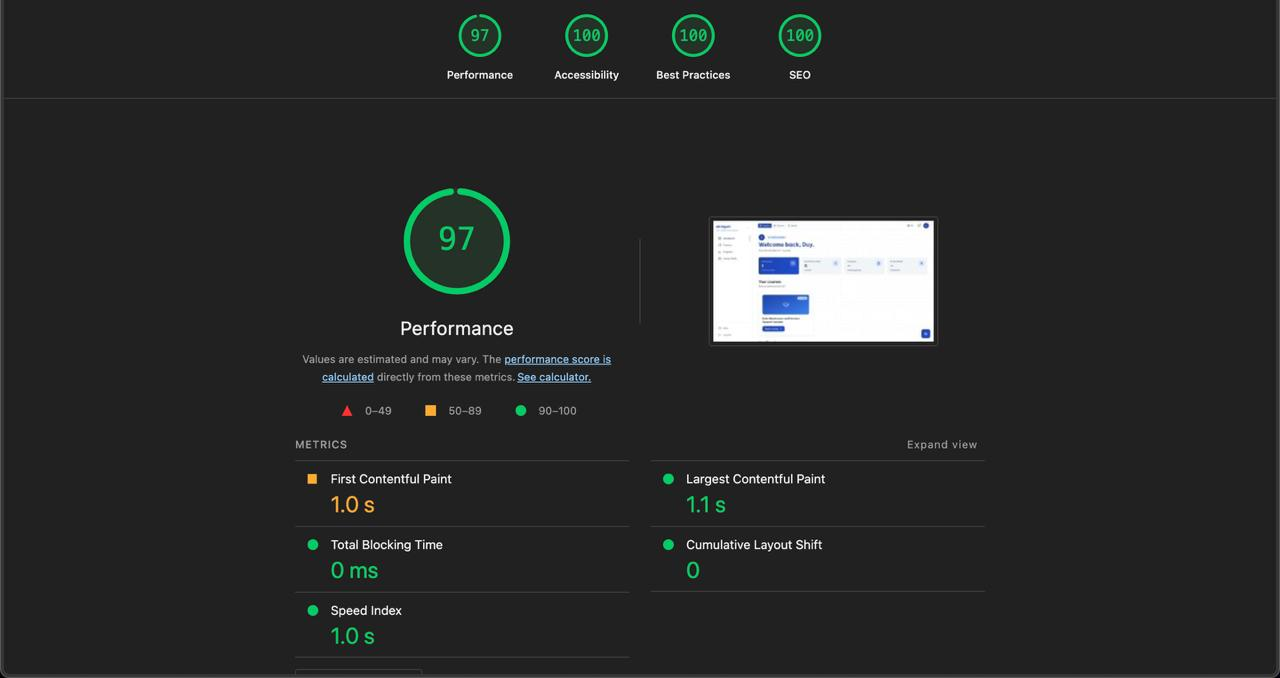
\includegraphics[width=0.85\textwidth]{graphics/lighthouse_dashboard.jpg}
    \caption{Lighthouse audit results for the Student Dashboard.}
    \label{fig:lighthouse_dashboard}
\end{figure}

Key performance metrics:
\begin{itemize}
    \item First Contentful Paint (FCP): 1.0\,s
    \item Largest Contentful Paint (LCP): 1.1\,s
    \item Total Blocking Time (TBT): 0\,ms
    \item Cumulative Layout Shift (CLS): 0
    \item Speed Index: 1.0\,s
\end{itemize}

Both pages achieve scores above 95 in all categories, confirming compliance with WCAG~2.1 AA accessibility standards (NFR-4.2) and adherence to web platform best practices.

% ===========================================================
\subsection{Backend Performance}
\label{sec:eval_backend}

Backend performance is evaluated using k6, an open-source load testing tool, targeting the deployed API at the development server. Tests measure response latency (p50, p95, p99), throughput (requests per second), and error rate under increasing concurrent load up to 100 virtual users (VUs).

\subsubsection{Test Environment}

\begin{itemize}
    \item \textbf{Server}: Development machine, single Uvicorn instance
    \item \textbf{Runtime}: FastAPI + Uvicorn, PostgreSQL 16, Redis 7
    \item \textbf{Load generator}: k6 v0.55 running from a separate machine on the same LAN
    \item \textbf{Protocol}: HTTP (no TLS overhead between load generator and server)
    \item \textbf{Authentication}: Pre-obtained JWT token (Google OAuth login is not load-tested due to external dependency)
\end{itemize}

\subsubsection{Test Scenarios}

Three scenarios are executed, each sustaining 100 concurrent virtual users for 30 seconds:

\begin{enumerate}
    \item \textbf{Health Check} (baseline) --- \path{GET /api/v1/healthz}. Measures pure framework overhead with no database or business logic.
    \item \textbf{Course Catalog} --- \path{GET /api/v1/courses}. Measures authenticated read-heavy list queries with cursor-based pagination against PostgreSQL.
    \item \textbf{Quiz Operations} --- \path{GET /api/v1/quizzes/{id}} and \path{GET /api/v1/me/quizzes/{id}/attempts}. Measures student-facing quiz detail retrieval and attempt history listing.
\end{enumerate}

\subsubsection{Results}

Table~\ref{tab:k6_results} presents the load test results under 100 concurrent users.

\begin{table}[htbp]
\centering
\caption{Backend Load Test Results (100 VUs, 30\,s sustained)}
\label{tab:k6_results}
\renewcommand{\arraystretch}{1.3}
\begin{tabular}{|l|c|c|c|c|c|}
\hline
\textbf{Scenario} & \textbf{p50} & \textbf{p95} & \textbf{Max} & \textbf{RPS} & \textbf{Error\%} \\
\hline
Health Check    & 135\,ms & 222\,ms & 445\,ms & 431 & 0\% \\
Course Catalog  & 207\,ms & 502\,ms & 737\,ms & 136 & 0\% \\
Quiz Operations & 214\,ms & 449\,ms & 1.18\,s & 159 & 0\% \\
\hline
\end{tabular}
\end{table}

\subsubsection{Analysis against NFR Targets}

\begin{itemize}
    \item \textbf{NFR-2.1} (50 concurrent users without performance degradation): \textbf{Exceeded.} The system handles \textbf{100 concurrent users} with 0\% error rate across all scenarios. Median response times remain below 215\,ms, and p95 latency stays under 510\,ms. This is double the specified NFR-2.1 target of 50 concurrent users.
    \item \textbf{Throughput}: The system sustains 136--431 requests per second depending on query complexity, confirming adequate capacity for the target 50-user workload.
    \item \textbf{Bottleneck}: The course catalog and quiz operations show similar latency profiles (p50 $\approx$ 210\,ms), suggesting the database query layer is the primary latency contributor rather than framework overhead (health check p50 = 135\,ms).
\end{itemize}

% ===========================================================
\subsection{AI Model Comparison for Quiz Generation}
\label{sec:eval_ai_model}

The quiz generation pipeline supports multiple LLM backends via the LLM Gateway abstraction. This section evaluates model performance for the quiz generation task across quality, latency, and cost dimensions to determine the optimal production default.

\subsubsection{Methodology}

Three candidate models were compared on a benchmark of two lessons from the \textit{Data Warehousing \& Data Mining} course (Chapter~1: Overview, Chapter~2: Basic Issues), running each model 3~times $\times$ 12~questions $\times$ 2~lessons = 72 expected questions per model. A JSON-repair fallback (via \texttt{gpt-5-chat-latest} with a structure-only system prompt) recovers malformed outputs, bringing all models to full sample size ($n = 72$ for gpt-oss and gemma, $n = 77$ for llama due to over-generation).

\paragraph{Generation parameters}
\begin{itemize}
    \item Temperature $= 0.3$, top\_p $= 0.95$
    \item 12 questions per lesson, fixed Bloom taxonomy mix (60\% remember, 30\% understand, 10\% apply)
    \item Same prompt template, same retrieved chunks, same JSON schema across all candidates
    \item Direct LLM gateway call (bypassing ARQ) to isolate the model effect from queue latency
\end{itemize}

\paragraph{Judge protocol}
An independent judge model (\texttt{gpt-5-chat-latest}) evaluated each generated question using a \textbf{reference-guided chain-of-thought} protocol~\cite{zheng2023llmjudge}:
\begin{enumerate}
    \item \textbf{Independently solve} the question using only the source chunks.
    \item \textbf{Compare} the independent answer with the marked-correct option and the candidate's explanation.
    \item \textbf{Score} the rubric only after Steps 1--2.
\end{enumerate}

This protocol reduces judge failure rates from 14/20 (default prompt) $\to$ 6/20 (plain CoT) $\to$ 3/20 (reference-guided), as reported in Table~4 of Zheng et al.~\cite{zheng2023llmjudge}. Anti-bias guardrails counter position, verbosity, and self-enhancement biases catalogued in~\cite{zheng2023llmjudge,li2024llmjudgesurvey}.

The judge scores each question on:
\begin{itemize}
    \item \textbf{Groundedness} (strict: explicit textual support required from source chunks)
    \item \textbf{Answer correctness} (does the marked-correct option match the source material?)
    \item \textbf{Judge-solve match} (fraction where the judge's independent answer matches the marked-correct option --- structural reliability check)
    \item \textbf{Distractor plausibility} (1--5 scale: 1 = trivially eliminable, 5 = requires deep understanding to distinguish)
    \item \textbf{Overall quality} (1--10 single-answer scale per Zheng et al.~\cite{zheng2023llmjudge} Figure~6)
    \item \textbf{Schema compliance} (valid JSON output parseable by the pipeline)
\end{itemize}

Confidence intervals are 95\% non-parametric bootstrap (2,000 resamples at question level). Decoding: temperature $= 0.0$, greedy (standard for LLM-as-a-judge stability~\cite{zheng2023llmjudge}).

\subsubsection{Quality Results}

Table~\ref{tab:model_quality} presents the quality evaluation results under the reference-guided judge protocol.

\renewcommand{\arraystretch}{1.3}
\begin{table}[htbp]
\centering
\caption{Quiz Generation Quality by Model (judge: \texttt{gpt-5-chat-latest}, reference-guided CoT)}
\label{tab:model_quality}
\begin{tabular}{|l|c|c|c|}
\hline
\textbf{Metric} & \textbf{gpt-oss-120b} & \textbf{gemma-4-31b-it} & \textbf{llama-3.3-70b} \\
\hline
Sample size ($n$)           & 72  & 72  & 77  \\
Groundedness (strict)       & 94.4\% & \textbf{100\%} & 77.9\% \\
Answer correctness          & 93.1\% & \textbf{100\%} & 84.4\% \\
Judge-solve match           & 93.1\% & \textbf{100\%} & 84.4\% \\
Distractor plausibility     & \textbf{4.07} & 3.86 & 3.97 \\
Overall quality (1--10)     & 8.62 & \textbf{8.97} & 8.04 \\
Schema compliance           & \textbf{100\%} & \textbf{100\%} & \textbf{100\%} \\
\hline
\end{tabular}
\end{table}

\textbf{Remark.} gemma-4-31b-it achieves perfect scores on all fidelity metrics --- the judge independently arrived at gemma's answer for every question (100\% solve-match), the strongest reliability signal available under reference-guided judging. gpt-oss-120b's 5.6~pp gap to gemma is attributable to paraphrasing depth rather than factual hallucination: when the judge could not solve a question, it also flagged it as not-grounded.

\subsubsection{Latency and Cost}

Table~\ref{tab:model_latency} presents latency per lesson (12 questions generated per call) and cost per 100 questions.

\begin{table}[htbp]
\centering
\caption{Quiz Generation Latency and Cost by Model}
\label{tab:model_latency}
\renewcommand{\arraystretch}{1.3}
\begin{tabular}{|l|c|c|c|}
\hline
\textbf{Metric} & \textbf{gpt-oss-120b} & \textbf{gemma-4-31b-it} & \textbf{llama-3.3-70b} \\
\hline
Mean latency / lesson       & \textbf{32.6\,s} & 125.6\,s & 81.6\,s \\
p99 latency / lesson        & \textbf{43.5\,s} & 140.9\,s & 95.0\,s \\
Per-question latency (p50)  & \textbf{2.7\,s} & 10.8\,s & 7.7\,s \\
Cost / 100 questions        & \textbf{\$0.0077} & \$0.0172 & \$0.0100 \\
\hline
\end{tabular}
\end{table}

\textbf{Remark.} gpt-oss-120b dominates on both latency (4$\times$ faster) and cost (2.2$\times$ cheaper than gemma). Per-question latency of 2.7\,s enables real-time generation feedback, whereas gemma's 10.8\,s requires an asynchronous queue pattern.

\subsubsection{Failure Analysis}

Each model exhibits distinct failure patterns under the reference-guided judge:

\paragraph{gpt-oss-120b} (production default)
Primary failure mode is \textit{paraphrase-depth}: the model rephrases source material at a level the judge's Step-1 solve cannot independently reproduce from the chunks alone ($\approx$5.6\% of questions). These are not factual hallucinations --- the judge's groundedness and solve-match failures overlap perfectly, confirming the issue is inference depth rather than content drift.

\paragraph{gemma-4-31b-it} (highest fidelity)
`Zero quality failures across all dimensions. The trade-off is distractor plausibility (3.86 vs gpt-oss's 4.07): gemma writes distractors that are \textit{too obviously wrong} for a learner familiar with the source, reducing exam discrimination power. One raw output required JSON structural repair (trailing prose after closing brace), recovered by the repair pass.

\paragraph{llama-3.3-70b} (not recommended for production)
Exhibits \textit{external-knowledge contamination} in $\approx$22\% of questions: the model injects pre-training knowledge (e.g., naming specific vendors not in the source), overgeneralises concepts beyond source scope, or confabulates examples. The reference-guided judge correctly identifies these because its Step-1 solve fails to land on llama's marked-correct option.

\subsubsection{Recommendation}

\textbf{Production default: gpt-oss-120b.} Fastest (4$\times$), cheapest (2.2$\times$), schema-perfect, highest distractor plausibility. Its 94.4\% strict groundedness approaches gemma's 100\% under reference-guided judging --- the gap is paraphrasing style, not factual error.

\textbf{High-stakes fallback: gemma-4-31b-it.} For graded assessments where any ungrounded content is unacceptable, gemma's perfect fidelity justifies the latency and cost premium. Schema fragility is mitigated by the JSON-repair pipeline.

All three models under-deliver on Bloom's \texttt{apply}-level questions (target 10\%, actual $<$2\%). This is addressable at the prompt level with worked examples, independent of model choice.

